

\chapter[High-fidelity and comprehensive DMS framework]{A framework for comprehensive and high-fidelity Deep Mutational Scanning}

\section{Introduction}

Within coming decades, millions of people will have their genome sequenced. Unfortunately, we have limited ability to interpret personal genomes, each carrying 100-400 rare missense variants~\cite{the_1000_genomes_project_consortium_global_2015} of which many must currently be classified as ``variants of uncertain significance'' (VUS). For example, gene panel sequencing aimed at identifying germline cancer risk variants in families yielded VUS for the majority of missense variants~\cite{maxwell_evaluation_2016}.  While functional variants can be predicted via computational tools such as PolyPhen-2~\cite{adzhubei_method_2010} and PROVEAN~\cite{choi_fast_2012}, these methods can confidently detect only one third as many disease variants as are detectable by experimental assays~\cite{sun_extended_2016}. Unfortunately, experimental assays are either unavailable or economically inviable for most human disease genes. The development of Deep Mutational Scanning (DMS)~\cite{fowler_high-resolution_2010} is making it possible to produce maps that predict the functional impact of a large fraction of substitutions for at least a subset of residue positions. Recently, Starita and colleagues carried out a DMS screen for the critical RING domain of BRCA18~\cite{starita_massively_2015}. Despite this progress, no experimental sequence-function map has yet demonstrated high-accuracy scoring of the functional impact of all possible substitutions for any full length protein (see Table~\ref{table:DMSstudies}). Thus, the goal of complete, highly accurate DMS maps for full-length proteins remains undemonstrated.

Functional complementation can measure the ability of a mutant human protein to rescue the loss of the wild type enzyme (or its ortholog in the case of trans-species complementation)~\cite{9,10}. We have previously found that cell-based functional complementation assays facilitated highly accurate identification of disease variation across a diverse collection of human disease genes~\cite{sun_extended_2016}. 

Here we describe a modular DMS framework to generate maps of variant function. The framework employs a novel mutagenesis strategy, functional complementation, two alternative sequencing-based selection screens, and a machine learning strategy that completes and refines the map via imputation and regularization. We first evaluate our framework on the SUMO E2 conjugase UBE2I.

\section{Results}

To carry out deep mutational scans of protein sequences yielding comprehensive atlases of sequence-function relationships, we found it useful to organize the process into six stages (see Figure~\ref{fig:framework}): 1) mutagenesis; 2) generation of a clone library; 3) selection for clones encoding a functional protein; 4) read-out of the selection results and analysis to produce an initial sequence-function map; 5) computational analysis to impute missing values; and 6) computational analysis to refine measured values based on imputation models. This framework incorporates previously-described deep mutational scanning concepts as well as new experimental components (e.g., our saturation codon mutagenesis strategy) and analytic methods.  The last two stages enabling a complete and accurate DMS map have not been applied in any published DMS study.

We first describe a variant of the framework called DMS-BarSeq and apply it to the human SUMO conjugase UBE2I, exhaustively measuring the ability of protein variants to function and to physically interact with protein partners.  Next, we describe a more efficient DMS-TileSeq variant of the framework, and apply this to UBE2I.  Having combined these maps, we computationally infer missing data points and refine map quality.


\begin{figure}[h!]
	\centering
	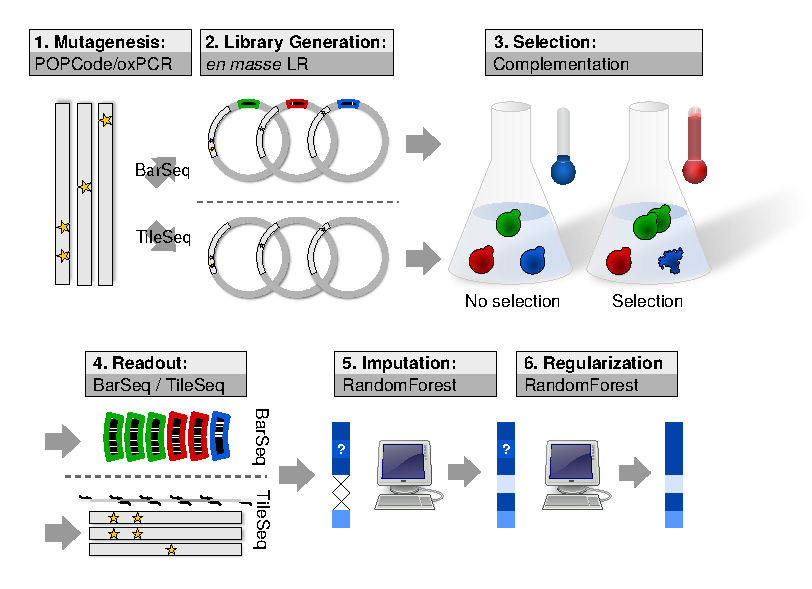
\includegraphics[width=\textwidth]{img/framework_flowchart.pdf}
	\caption{An overview of the Deep Mutational Scanning Framework.}
	\label{fig:framework}
\end{figure}


\subsection{A barcode-based Deep Mutational Scanning strategy}

%Describe goals for this screen, and then how the different choices below aim to achieve these.

As an initial test of the overall framework, we first aimed to generate a map of functional missense variation for UBE2I. Our goals for this map were as follows: (i) High and even coverage of the full spectrum of amino acid changes;(ii) Determination of mutant effects on overall protein functionality; (iii) High fidelity of functional effect readouts. We therefore designed the different stages of the framework accordingly. 

For Stage 1 of the DMS framework---mutagenesis--- to achieve a relatively even representation of all possible single amino acid substitutions, we wished to allow multiple mutations per clone. This would not only allow for greater mutational coverage for any given library size, but it would also offer an opportunity to discover intragenic epistatic relationships between variants.  To fulfill these requirements, we developed a mutagenesis protocol (Precision Oligo-Pool based Code Alteration or POPCode) which generates random codon replacements. 
At the second stage---library generation---we wished to be able to track the fitness effects of each individual mutant clone rather than just average effects of mutations across the population, as this could be expected to allow for higher quality measurements. Thus, in Stage 2 of the framework, we opted to assign molecular barcodes to each clone that could be identified by sequencing. To catalogue the pairing of mutant genotypes with barcodes, we developed a novel multiplex amplicon sequencing method called KiloSEQ, in collaboration with SeqWell Inc, Boston. 
The selection process (Stage 3) was performed as a yeast complementation assay, to allow for determination of overall functional effects of mutations. The assay would be performed as a time series in triplicates, as this again promised to allow for higher quality of readouts 
Finally, Stage 4, would consiste of barcode sequencing and statistical analysis. All four stages will be described in further detail in the following subsections.


\subsubsection{POPCode: A Precision Oligo Pool Codon alteration mutagenesis method}

This method scales up a previously described method developed by Seyfang~\etal~\cite{seyfang}. To achieve complete wide coverage over the complete spectrum of possible amino acid changes we design oligonucleotides centering on each codon in the Open Reading Frame (ORF) of interest and replacing the target with an \texttt{NNK} degeneracy code. This has been previously demonstrated to allow all amino acid changes while reducing the chance of generating stop codons~\cite{36}. 
In the next step, the ORF sequence is PCR amplified in the presence of dUTP to generate uracil-doped template for the mutagenesis reaction. Oligonucleotide pools were then hybridized with the template. Gaps between hybridizations were filled and sealed with the non-strand-displacing \species{Sulpholobus} Polymerase~IV. 

When finding a set of suitable oligonucleotide sequences, two important criteria need to be considered: 
(i) The melting temperature across the complete set is as uniform as possible as this will ensure a more even mutation rate across the ORF sequence; (ii) the degenerate codon sequence should be located as close to the center of the oligo as permissible given the first criterium. To simplify the process of choosing an appropriate set of oligos based on these criteria I developed a web tool that can be used to calculate the optimal solution to the given problem. The tool merely requires the sequence of the target ORF and flanking vector sequences, a desired average oligo length and a maximum offset parameter. The offset parameter determines how many bases can be maximally added or removed from each side of a given oligo to optimize its melting temperature. 

In some cases a moderate deviation from the average in melting temperature for some oligos cannot be avoided. To alleviate these effects, the webtool also offers a mutation rate prediction. This is based on observations from all the POPCode procedures performed as part of this work in combination with linear regression. The prediction can be used to preemptivly adjust concentrations of potentially troublesome oligos in the POPCode protocol. An additional webtool feature based on the mutation rate prediction is the automatic calculation of necessary library size to achieve a desired mutational coverage. The webtool as available at \verb|http://llama.mshri.on.ca/cgi/popcodeSuite/main|.

%%Figure: PopCode schema

\begin{figure}[h!]
	\centering
	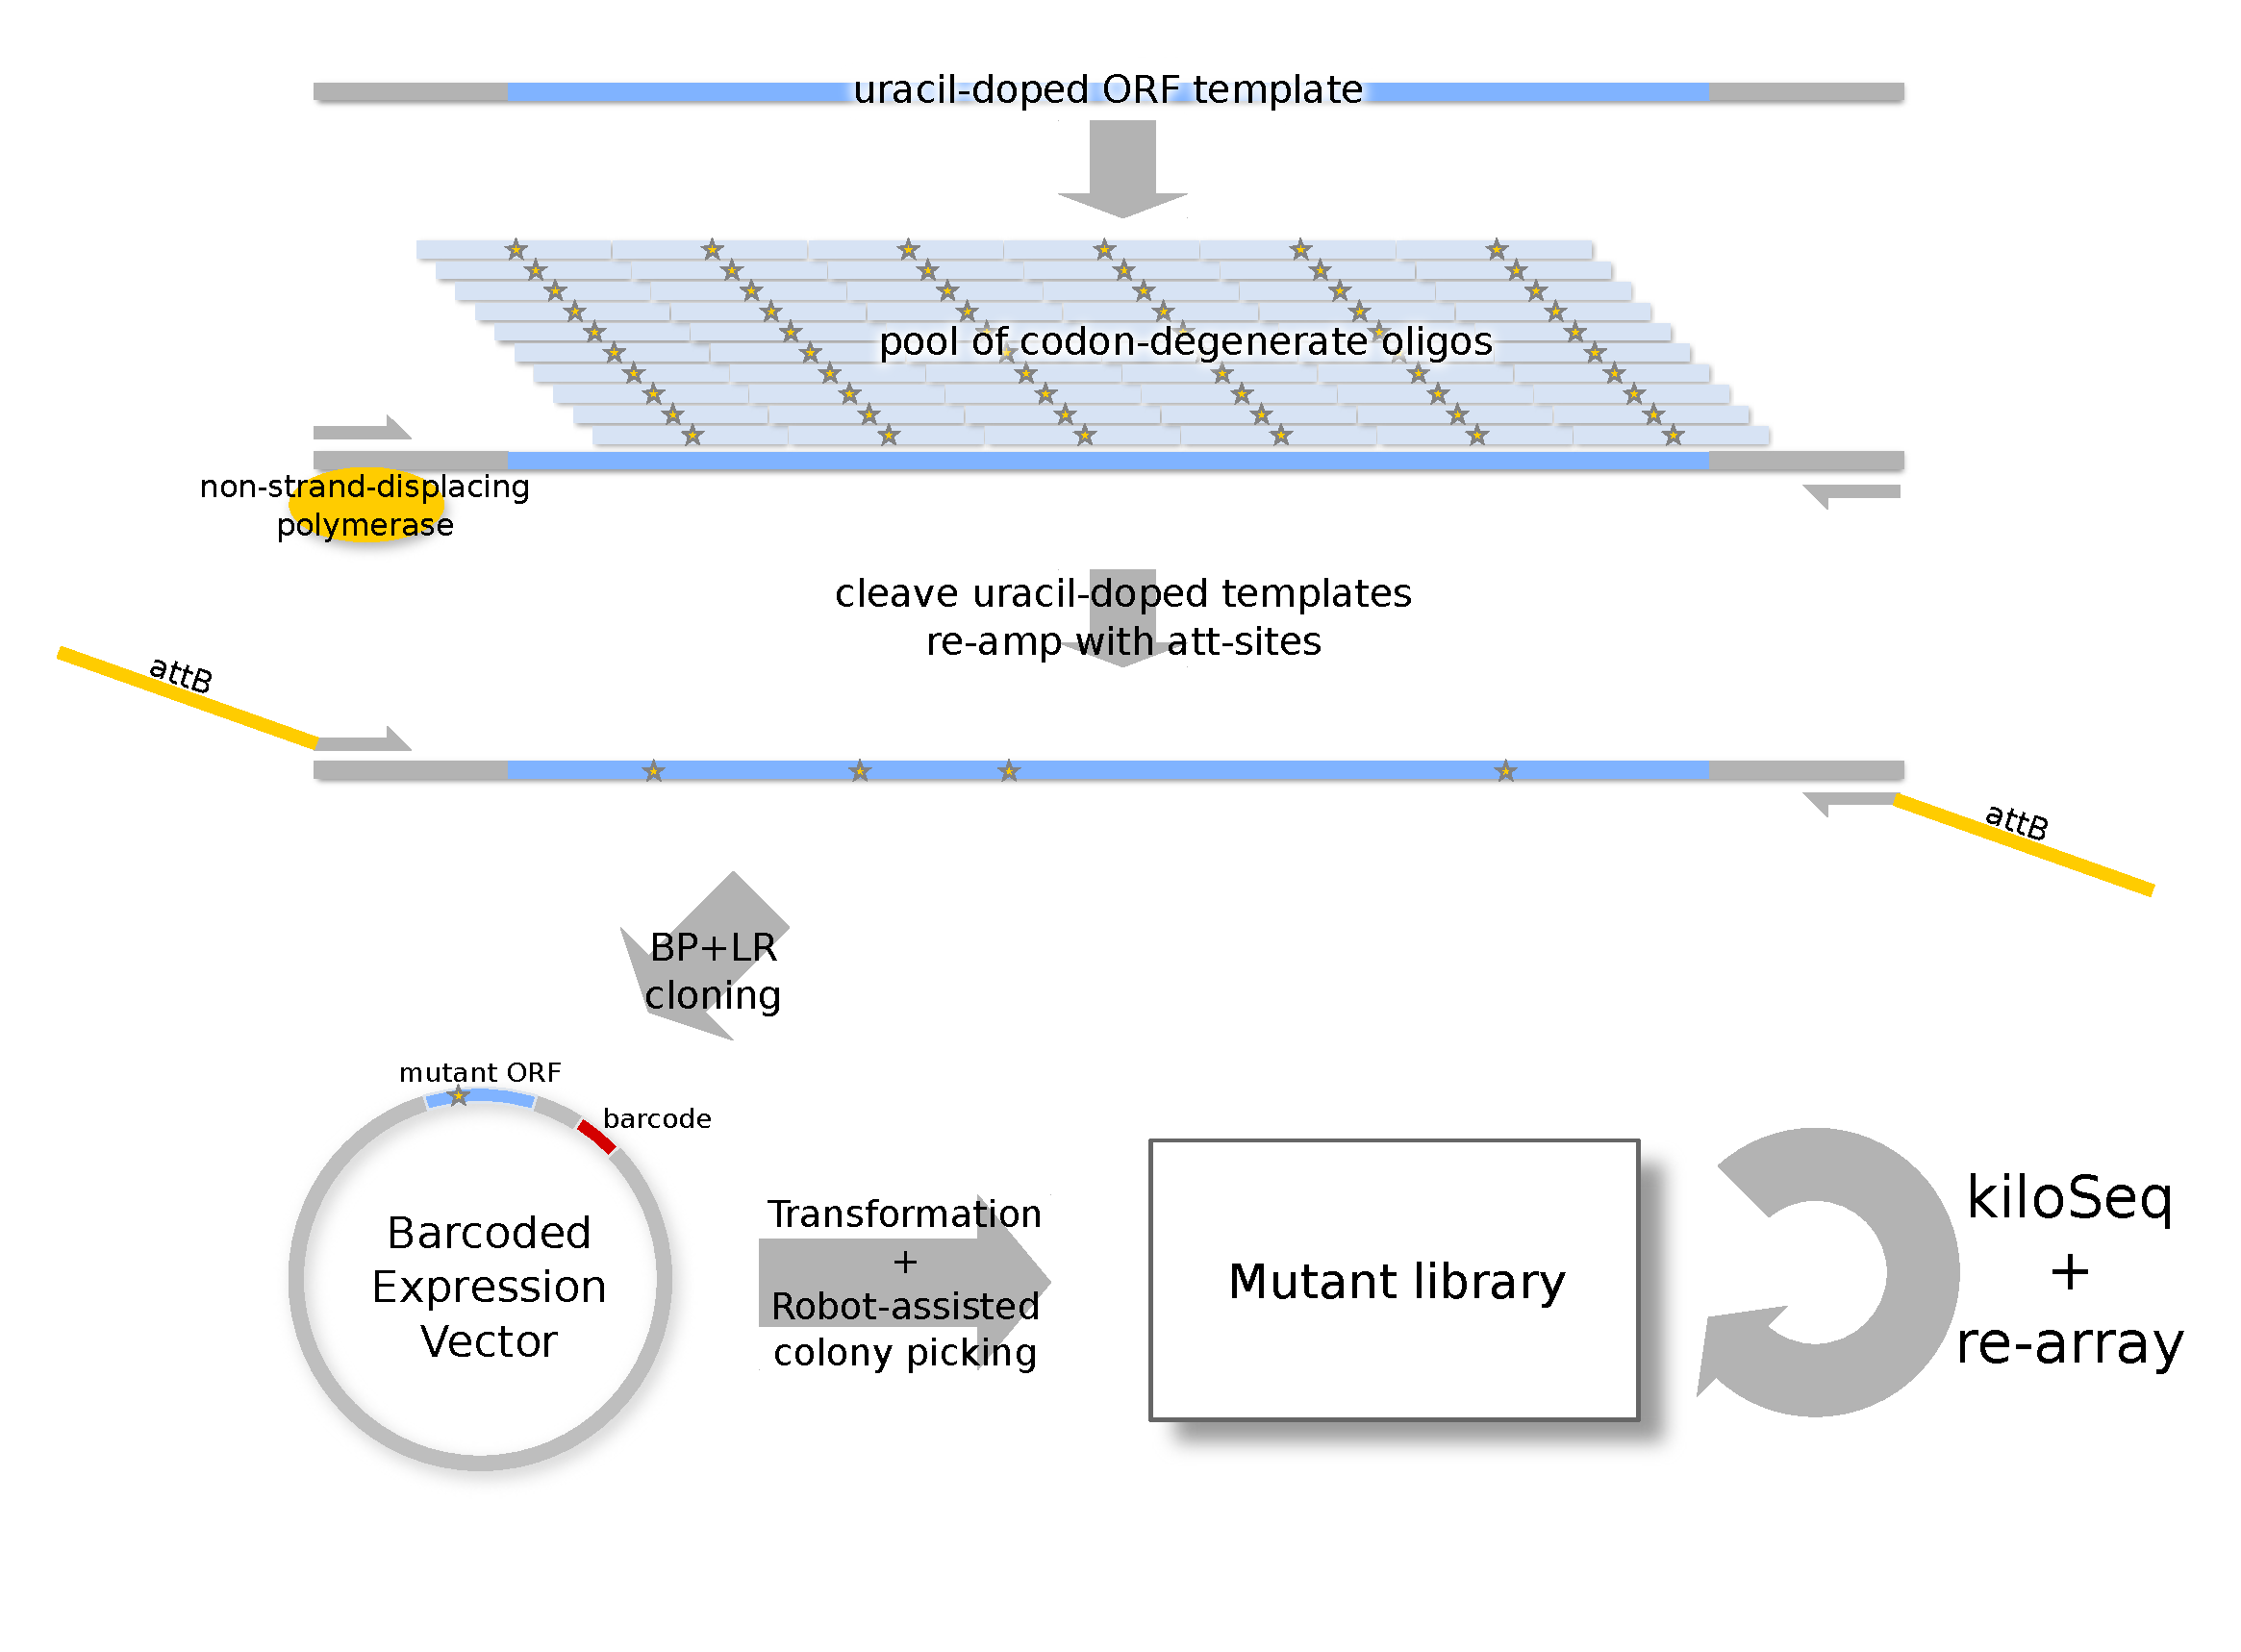
\includegraphics[width=\textwidth]{img/popcode_schema.pdf}%TODO: should be direct BP-LR cloning
	\caption{POPCode mutagenesis and library generation. A pool of codon-denerate oligos is hybridized to a uracil-doped template, gaps between oligos are closed via non-strand-displacing polymerase and the backbone sealed. Uracil-doped template is degraded to enrich for mutants. After mutagenesis, Gateway attB sites are added, followed by BP+LR cloning into barcoded vectors and transformation into bacteria. Finally, colonies are picked and arrayed.}
	\label{fig:popcode_schema}
\end{figure}
Following cleanup, the uracil-doped template was incapacitated using Uracil-DNA-Glycosylase (UDG). The mutagenesis product was then amplified with primers that added attB sites to allow Gateway BP cloning into entry vectors.

To accomplish mutagenesis across the entire coding region of our gene of interest, \gene{UBE2I}, we designed a tiled collection of oligos (one per codon) and applied POPCode to generate a codon-mutagenized amplicon library.  In parallel, we carried out PCR with oxidized nucleotides~\cite{oxPCR} to enable deeper representation of amino acid changes achievable from single-nucleotide changes.

\subsubsection{Library generation and highly multiplexed amiplicon sequencing}

For Stage 2 of the framework---generation of a clone library---we employed an \textit{en masse} recombinational cloning strategy to generate a Gateway Entry vector library of \gene{UBE2I} variants. This library was transferred via \textit{en~masse} recombinational subcloning into a pool of randomly-barcoded plasmids enabling expression of UBE2I variants in yeast. As sequencing is required to establish the full-length ORF sequence and barcode of each clone, the complementation vector is designed such that the variant ORF and the barcode locus are in close proximity to each other. Thus, only a relatively small segment of the plasmid needs to be inspected to determine the pairing of genotype and barcode. 

After bacterial transformation, we proceeded to robotically pick 19,968 colonies, which were stored in 52 384-well plates. As sequencing needs to be performed to catalogue the identities of nearly 20,000 individual samples, we used a novel sequencing method called KiloSEQ which combines plate-position-specific index sequences with Illumina sequencing (Figure~\ref{fig:kiloseq_schema}).
KiloSEQ was developed in collaboration with SeqWell Inc., Boston. First, for each clone in the library, the region of interest is amplified with primers containing well-specific tags, uniquely identifying each well coordinate. In the next step, wells for each plate can be pooled. Nextera tagmentation using Tn5 transposase is used to break the amplicons into random fragments and simultaneously ligate them to Illumina sequencing linkers with plate-specific indices. We then re-amplify the pool with  3'-specific primers, to enrich for fragments that contain the well tags. The resulting library is now ready for paired-end sequencing. In each pair of reads, one read will contain the well tag and the barcode locus, whereas the other will contain a fragment of the mutant ORF.
%TODO: move to methods: This is done using a hydrocycler, allowing for thousands of PCR reactions to be performed in parallel. ----- Amplicons can then be plate-wise pooled.

\begin{figure}[h!]
	\centering
	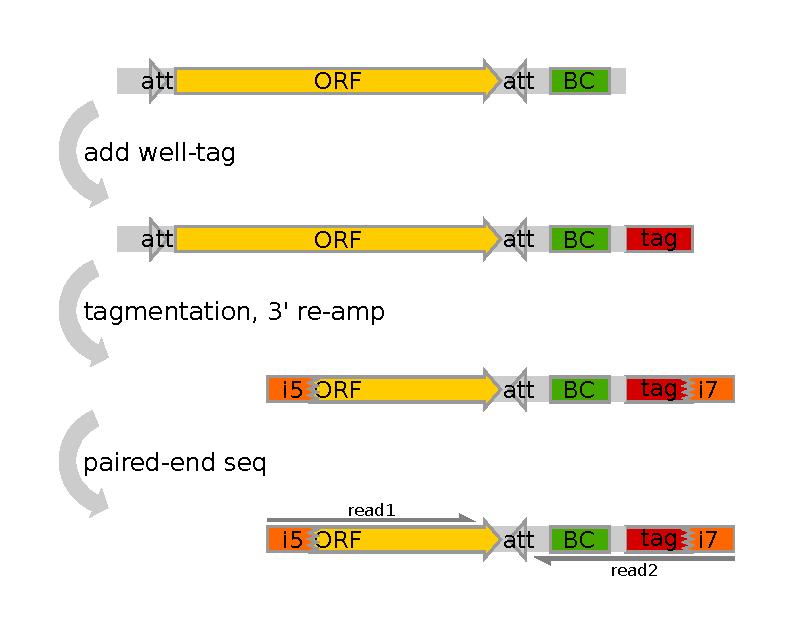
\includegraphics[width=.5\textwidth]{img/kiloseq_schema_new.pdf}
	\caption{KiloSEQ schema. 1) For each library well, amplicons containing the variant ORF (gold) and Barcode locus (green) are amplified with primers adding a well-specific tag. 2) Tn5 tagmentation fragments the DNA while simultaneously adding Illumina i5/i7 linkers. 3' re-amplification enriches for fragments containing the well tags. 3) Each pair of sequencing reads now contains a fragment of ORF sequence and the associated barcode and well tag.}
	\label{fig:kiloseq_schema}
\end{figure}

To process the results of a KiloSEQ sequencing run, a special software pipeline was developed, which can be divided into three phases: Demultiplexing; Barcode clustering; and Alignment and variant calling.
The first phase---demultiplexing---takes place on two levels, corresponding to library plates and the wells within those plates. Demultiplexing at plate level is performed by Illumina's bcl2fastq software, which resolves i5-i7 index combinations. The second phase is performed on a high performance computing cluster. Sets of read pairs are distributed across computing nodes, where they are processed by worker scripts. The well-tag within each R2 read is identified using a k-mer search algorithm, and read-pairs are sorted accordingly into bins. Each bin corresponds to one well in a given plate. At the same time, barcode sequences are extracted from the R2 reads in preparation for the next phase. 

The second phase---barcode clustering---uses the extracted barcode sequences within each bin and clusters them according to their Levenstein distance~\cite{Levenstein} (i.e. the number of edit operations required to transform one into the other). This step is necessary in order to resolve possible contamination across wells that occurred during library preparation. Each barcode cluster corresponds to a different clone, and the different unique sequences within each clusters correspond to different sequencing errors. The most frequently observed sequence within each cluster is interpreted as the true barcode. Finally, read pairs within each bin are again subdivided according to their respective barcode cluster.

The third phase---alignment and variant calling---is then executed for each barcode cluster within each well within each plate. The R1 reads are aligned to the template sequence and variants are called. This is complicated by the fact that the KiloSEQ library preparation usually creates a certain amount of cross-contamination between wells. While single or multi-nucleotide variants are still relatively unproblematic to identify, standard tools were found to be unable to identify copy number variations (CNVs) due to these problems. We thus developed a custom method for CNV calling, based on detecting sudden changes in read depth across the alignments. First the individual read depth track is normalized to the average read depth across the plate. Then a one-dimensional Sobel operator is used to detect sharp edges in the signal. An example of this can be seen in Figure~\ref{fig:border_detect}. Detection thresholds were optimized by comparison with Sanger sequencing.

\begin{figure}[h!]
	\centering
	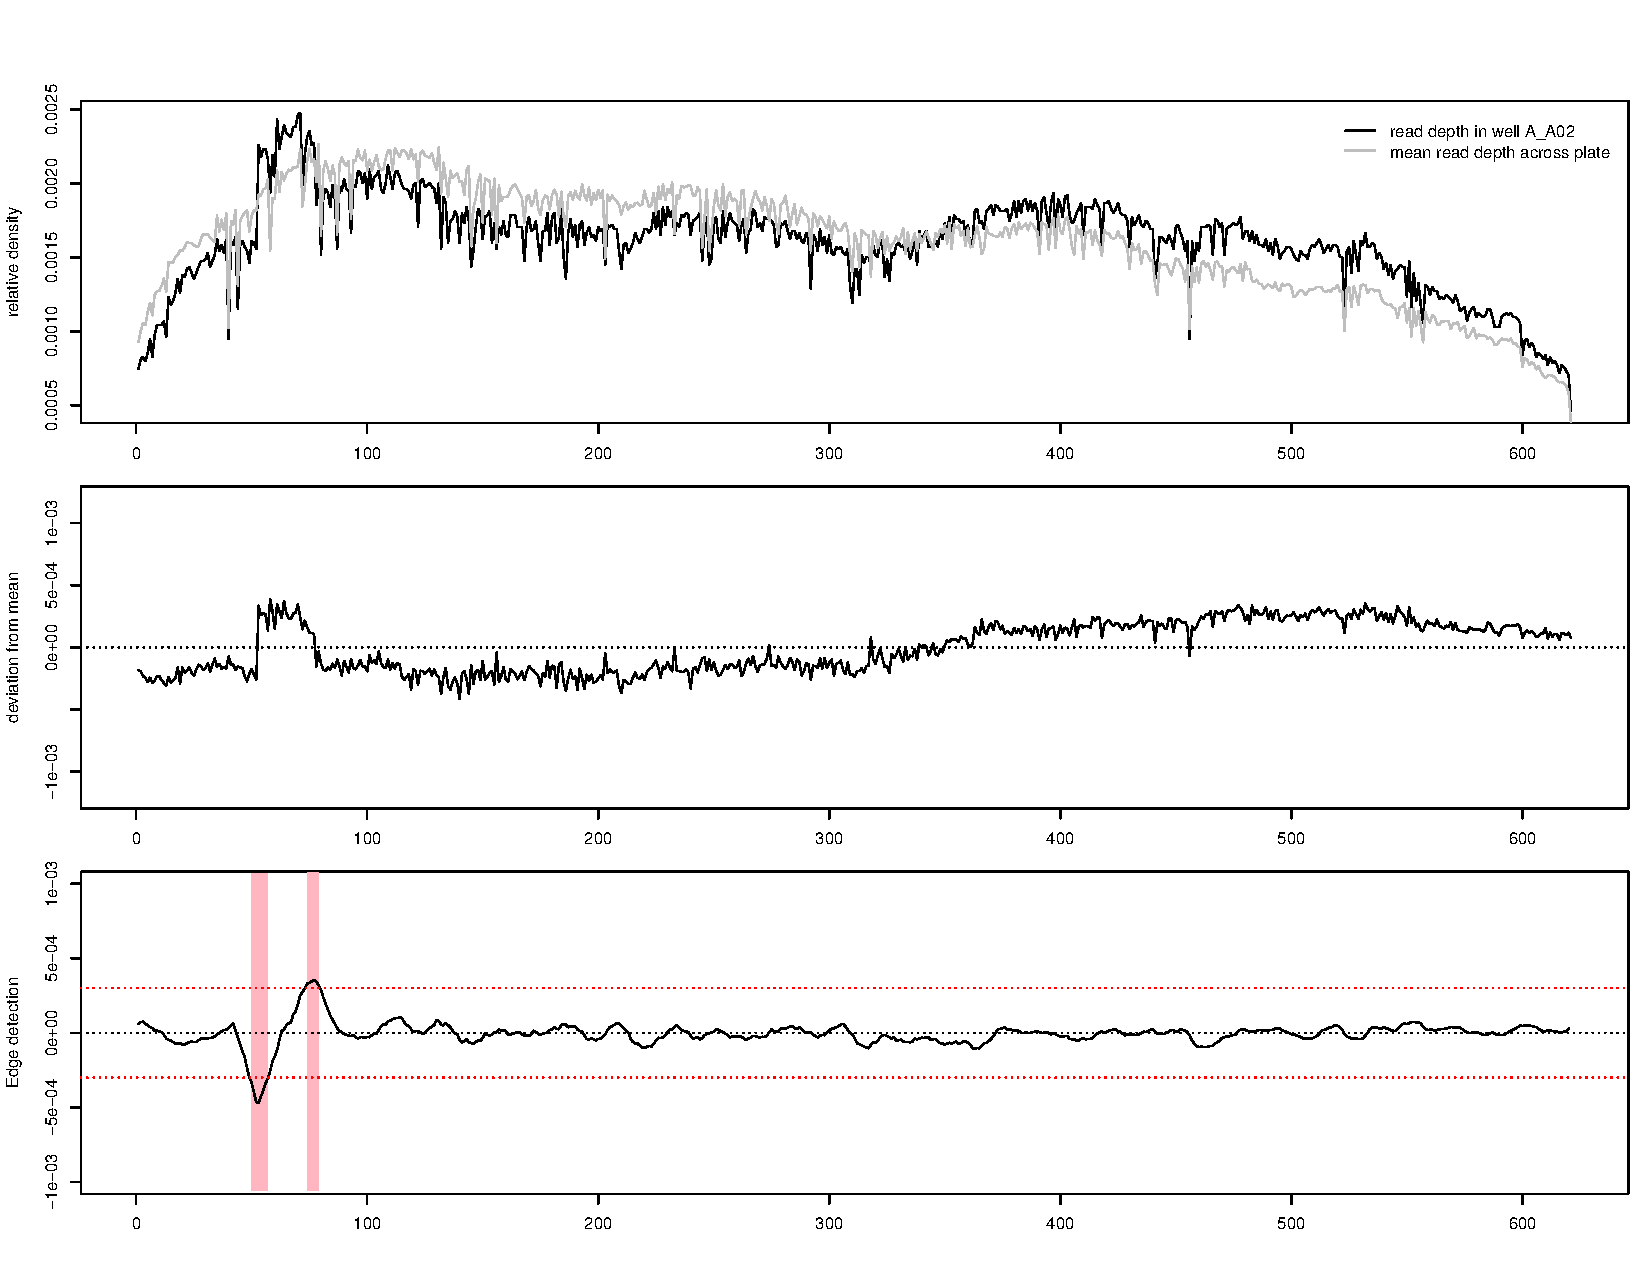
\includegraphics[width=\textwidth]{img/border_detect.pdf}
	\caption{Indel detection example. A duplication event in well \texttt{A\_A02} is detected by normalizing relative read depth by the mean depth across the plate and using a Sobel operator to detect sudden changes.}
	\label{fig:border_detect}
\end{figure}


After successful genotyping with kiloseq, we determined the subset of clones that (i) contained at least one missense mutation, (ii) did not contain any insertions or deletions, (iii) did not contain mutations outside of the ORF, (iii) had unique barcodes, (iv) had sufficient read coverage during kiloSEQ to allow for confident genotyping.
Over half of clones in the library conformed to these criteria. The single largest reason for exclusion was the occurrence of indels and CNVs (Figure~\ref{fig:popcode_census}A). 

An analysis of the mutation signatures across clones generated by POPCode revealed that two different mechanisms appear to underly mutagenesis. When considering only mutations that change more than one base in a given codon, there is an equal chance for every possible base except in the third position, where almost no adenine or cytosine was introduced. This is consistent with the NNK degeneracy code used in the POPCode oligo design. By contrast, variants that change only a single base in a given codon show a strong bias for transitions over transversions. These could be introduced due to polymerase error (Figure~\ref{fig:popcode_census}B). This is also reflected in the relative share of single nucleotide variants, which make up 56\% of mutations (Figure~\ref{fig:popcode_census}C). As a consequence, when examining the mutation coverage across the sequence of the ORF, it is clearly visible that the share of amino acids reachable with a single nucleotide change from the respective wildtype codon is much closer to saturation than the the set of all possible amino acid changes (Figure~\ref{fig:popcode_census}D). Additionally some hotspots are visible, in which mutation rate is higher, which is likely due to different hybridization efficiencies of oligos across the ORF sequence.

\begin{landscape}
\begin{figure}[h]
	\centering
	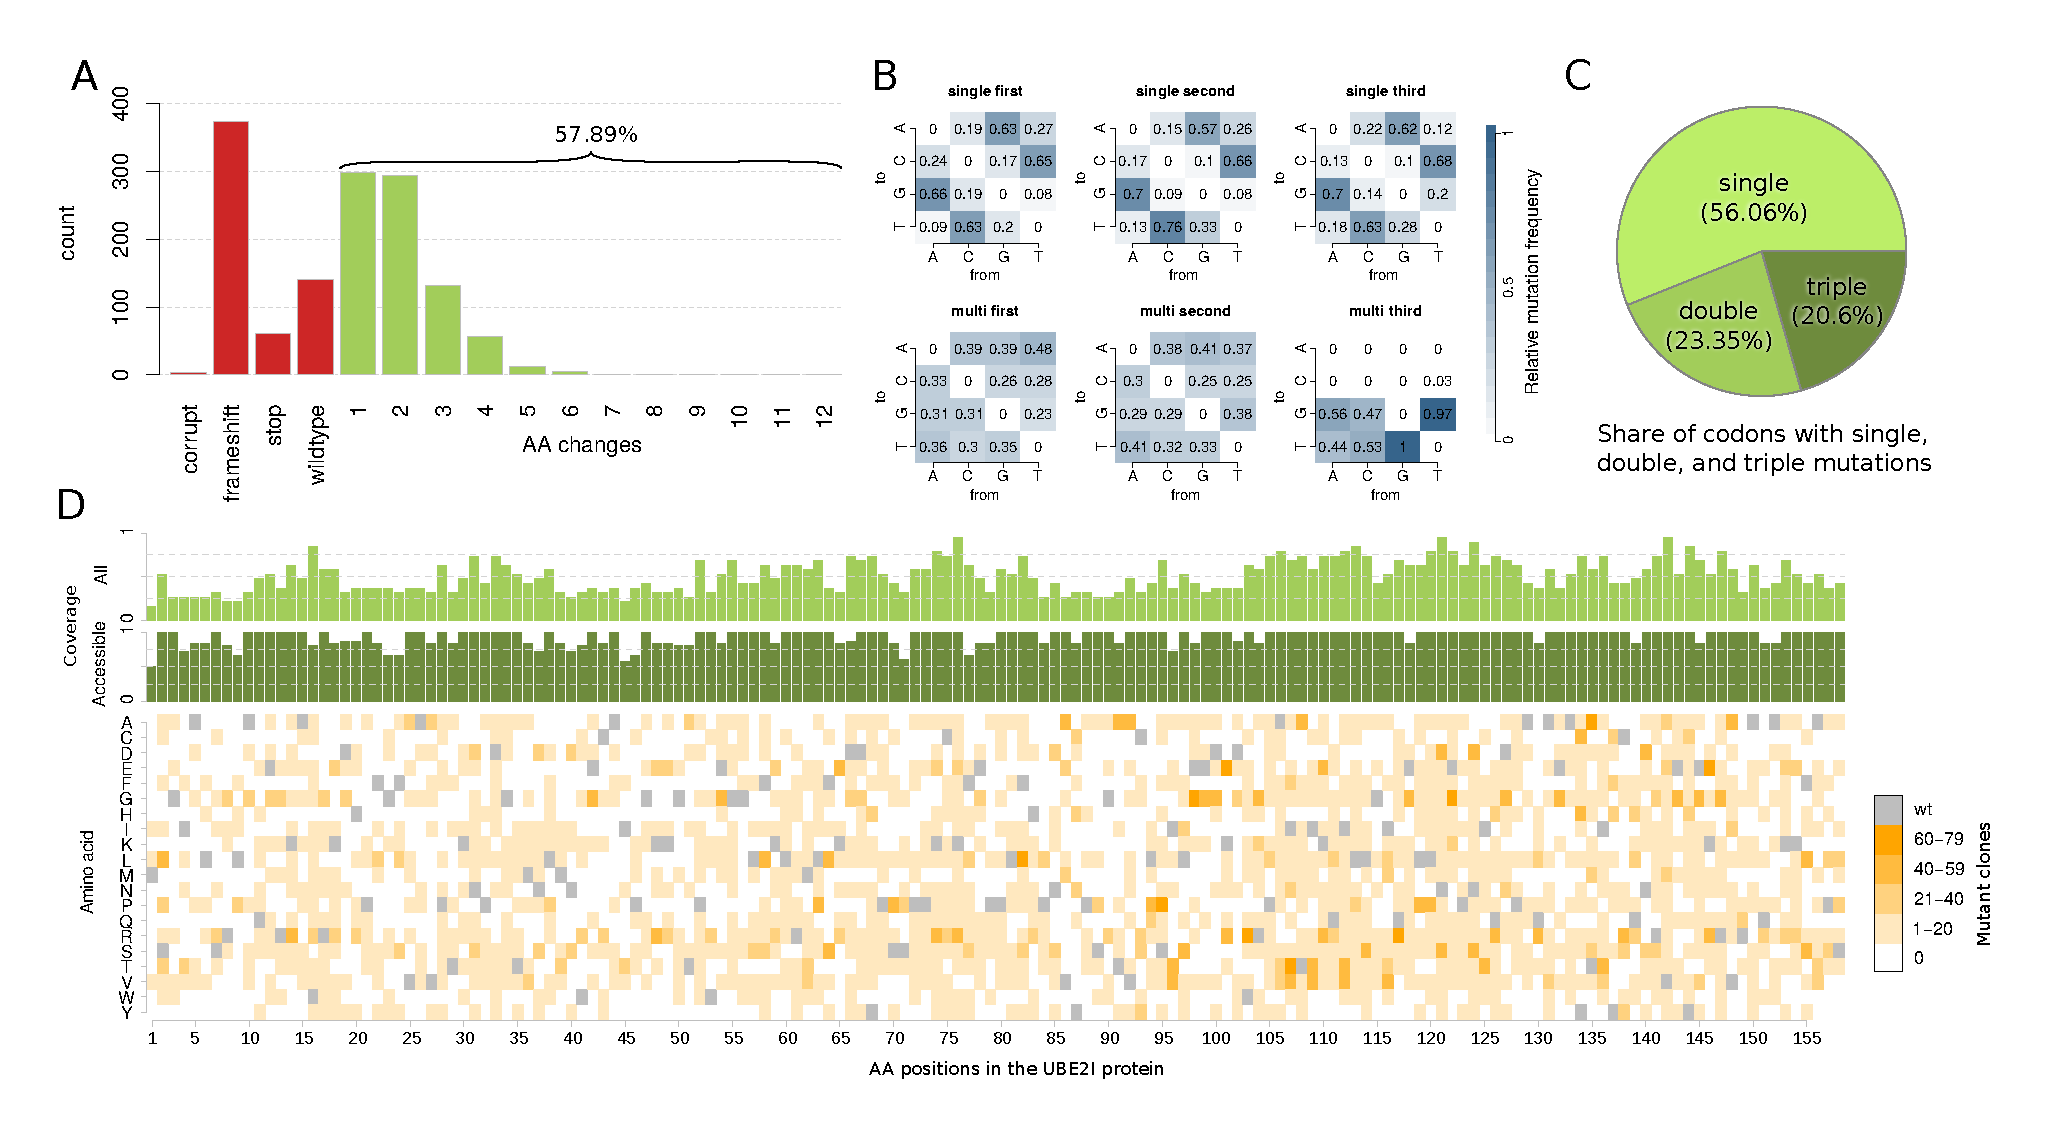
\includegraphics[width=9in]{img/popcode_census.pdf}
	\caption{KiloSEQ census of UBE2I POPCode library. A) Breakdown of KiloSEQ results for a set of five 384 well plates of mutant clones generated by POPCode. Corrupt: Clones containing mutations outside of the ORF; Frameshift: Clones containing indels or copy number variants; Stop: Clones containing stop codons. B) Breakdown of mutations in codons. Top: Single nucleotide variants; Bottom: Multi-nucleotide variants. Columns correspond to the first, second and third position in a codon. C) Relative shares of single, double and triple nucleotide variants among all missense variants in the library. D) Coverage map of missense variants in the library. Light green track: Coverage across all possible amino acids; Dark green track: Coverage across amino acids reachable with a single nucleotide change from the wildtype codon.}
	\label{fig:popcode_census}
\end{figure}
\end{landscape}

Using the Biomatrix robot, we re-arrayed the subset of usable clones into a condensed final library of 40 plates. This final library comprised 6,553 UBE2I variants, covering different combinations of 1,848 (61\% of all possible) unique amino acid changes. In preparation for the next stage, variant plasmids were pooled, together with barcoded empty vector and wild type control plasmids.


\subsubsection{Complementation screen and Barcode sequencing}

For Stage 3---the selection of clones encoding a functional protein---we employed a previously described \species{S.~cerevisiae} functional complementation assay~\cite{5,13}. This assay is based a yeast strain carrying a temperature sensitive (ts) allele of the UBE2I orthologue UBC9. Expression of human UBE2I rescues growth at an otherwise lethal elevated temperature. As such, the fitness observed for a clone carrying a mutant allele of UBE2I can be interpreted as the overall ability of the variant protein to function within its biological context~\cite{Song}. 
The plasmid library from Stage 3 was introduced into the appropriate ts strain by en-masse transformation. Pools were then grown in triplicates over a period of 48 hours at the permissive (25\celsius ) and selective (37\celsius ) temperatures, respectively (see Online Methods) and evaluated at multiple time points via high-throughput sequencing.

To facilitate the readout of the selection (Stage 4), I developed a sequence analysis pipeline. The pipeline distributes sets of read pairs across across the nodes of a high-performance computing cluster, where a k-mer search algorithm is used to identify multiplexing tags that encode the temperature and time point and replicate number associated with the sample. The same algorithm is also used to identify the barcode itself. The number of occurrences of each barcode in each sample is counted and aggregated across the cluster nodes. The frequencies at which each barcode is observed corresponds to the population size of the associated clone. This can then be used to reconstruct of individual growth curves and quantify the normalized fitness for each of the 6,553 strains as follows: Let $c_{i,t_k}^\tau$ be the barcode count for clone $i$, timepoint $t_k$ at temperature $\tau$, then $ \forall i \in \{1 \le i \le N | i \in \mathbb{N} \}$, 
$\forall k \in \{1 \le k \le 5 | k \in \mathbb{N} \}$, 
$\forall \tau \in \{25^{\circ},37^{\circ} \}$
\begin{align*}
r_{i,t_k}^{(\tau)} &= \frac{ c_{i,t_k}^{(\tau)} }{ \sum_j c_{j,t_k}^{(\tau)} }\\
P_{i,t_k}^{(\tau)} &= r_{i,t_k}^{(\tau)} \cdot P_{*,t_k}^{(\tau)} \\
\rho_{i,t_k}^{(\tau)} &= \sqrt[\uproot{5}(t_k - t_{k-1})]{\frac{P_{i,t_k}^{(\tau)}}{P_{i,t_{k-1}}^{(\tau)}}} \\
%\rho_{*,t_k}^\tau &= \sqrt[\uproot{5}(t_k - t_{k-1})]{\frac{P_{*,t_k}^\tau}{P_{*,t_{k-1}}^\tau}} \\
\phi_{i,t_k}^{(\tau)} &= \frac{\rho_{i,t_k}^{(\tau)}}{\rho_{*,t_k}^{(\tau)}}\\
\phi_{i,t_k}^\prime &= \frac{\phi_{i,t_k}^{(37^{\circ})}}{\phi_{*,t_k}^{(25^{\circ})}}\\
s_i &= \prod_k \phi_{i,t_k}^\prime \\
s'_i &= \frac{s_i - s_\text{null}}{s_\text{wt} - s_\text{null}},
\end{align*}

where $r_{i,t_k}^{(\tau)}$ is the relative population size for clone $i$ and timepoint $t_k$ at temperature $\tau$, $P_{i,t_k}^{(\tau)}$ is the absolute population size for clone $i$, timepoint $t_k$ at temperature $\tau$, $\rho_{i,t_k}^{(\tau)}$ is the measured hourly growth rate for clone $i$, timepoint $t_k$ at temperature $\tau$, $\phi_{i,t_k}^{(\tau)}$ is the fitness advantage relative to the pool growth for clone $i$, timepoint $t_k$ at temperature $\tau$, $\phi_{i,t_k}^\prime$ is the normalized relative fitness advantage for clone $i$ at timepoint $t_k$, and $s_i$ is the cumulative normalized relative fitness advantage for clone $i$. Finally, $s'_i$ is the fitness score relative to the internal null and wild type controls. This results in null-like mutants receiving a score of zero and wild type-like mutants receiving a score of one.

Additional care needs to be taken to quantify the level of confidence for each fitness measurement. While comparing the three technical replicates available for each clone allows for a rough estimation of standard error, improvements can be made. Baldi and Long previously published a Bayesian method allowing for the regularization of variance estimations using prior data~\cite{baldiLong}. Two sources of prior information offer themselves: (1) A low number of reads counted at time 0 of the experiment which is likely to result in a poor frequency estimate; and (2) the fitness estimate itself, as variance is often proportional to the mean. Indeed, when comparing both properties with the standard deviation, a clear trend is visible (Figure~\ref{fig:baldiLong}). After obtaining a prior via linear regression, it can be used to regularize the empirical standard deviation estimate.

\begin{figure}[h!]
	\centering
	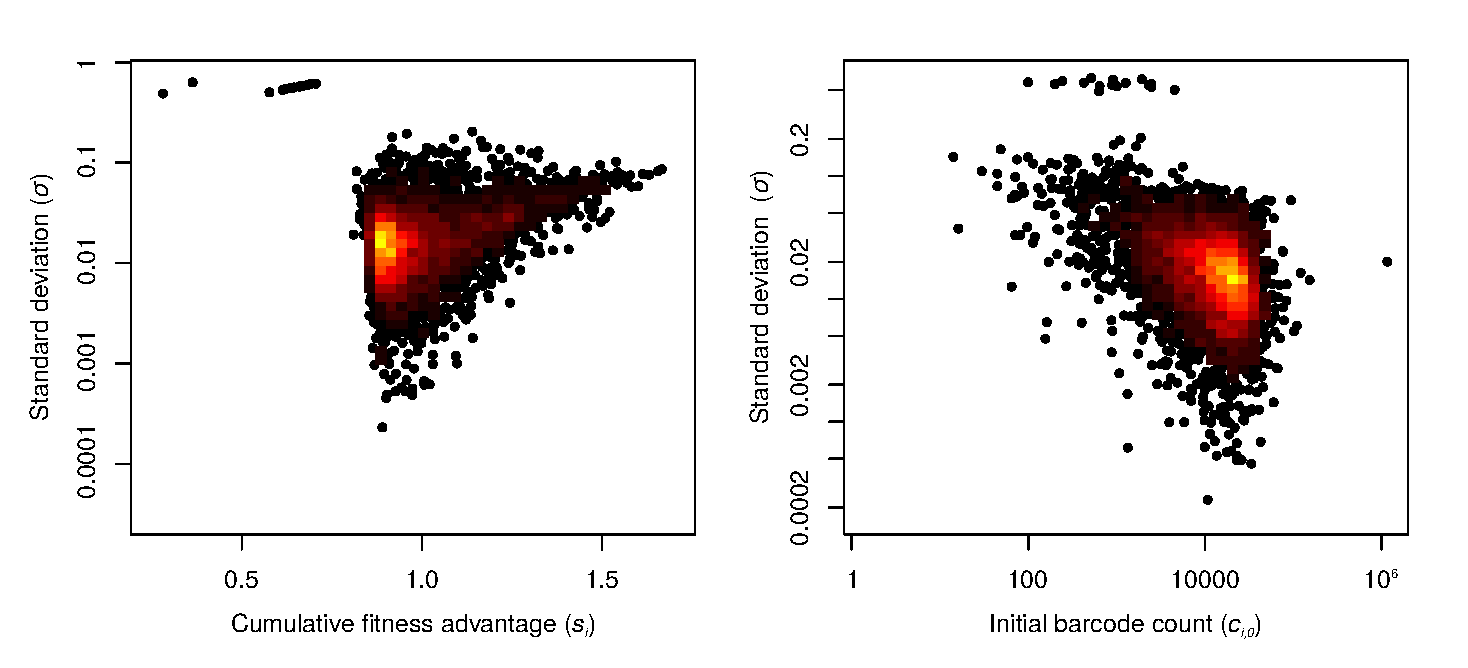
\includegraphics[width=\textwidth]{img/baldi_long.pdf}
	\caption{Comparison of fitness and initial barcode count against standard deviation. Both properties can be used as prior information to improve confidence quantification.}
	\label{fig:baldiLong}
\end{figure}


\subsubsection{A barcoded-based functional map of UBE2I}

Before further refinement in Stages 5 and 6, we wished to assess the quality of complementation scores. We first examined reproducibility of scores between technical replicates (Figure~\ref{fig:barseqValidation}A), and biological replicates (different clones carrying the same mutation; Figure~\ref{fig:barseqValidation}B).  In each case the scores were reproducible (Pearson’s R of 0.97 and 0.78, respectively). We next carried out semi-quantitative manual complementation spotting assays for a subset of mutants that spanned the range of fitness scores. Complementation scores from deep mutational scanning correlated well with these small-scale tests. Indeed, agreement between the large-scale and manual scores was about the same as agreement between internal replicates of the large-scale scores (Figure~\ref{fig:barseqValidation}B,C). 

As a further sanity check, we next examined evolutionary conservation and common predictors of deleteriousness, such as PolyPhen-2~\cite{polyphen} and PROVEAN~\cite{provean}.  Although each of these measures is far from perfect in predicting the functionality of amino acid changes, they should and did each correlate with functionality (Figure~\ref{fig:barseqValidation}D,E,F). Finally, we confirmed that, as expected, amino acid residues on the protein surface are more tolerant to mutation than those in the protein core or within interaction interfaces (Figure~\ref{fig:barseqValidation}G).  Taken together, these observations support the biological relevance of the DMS-BarSeq approach.

\begin{landscape}
\begin{figure}
	\centering
	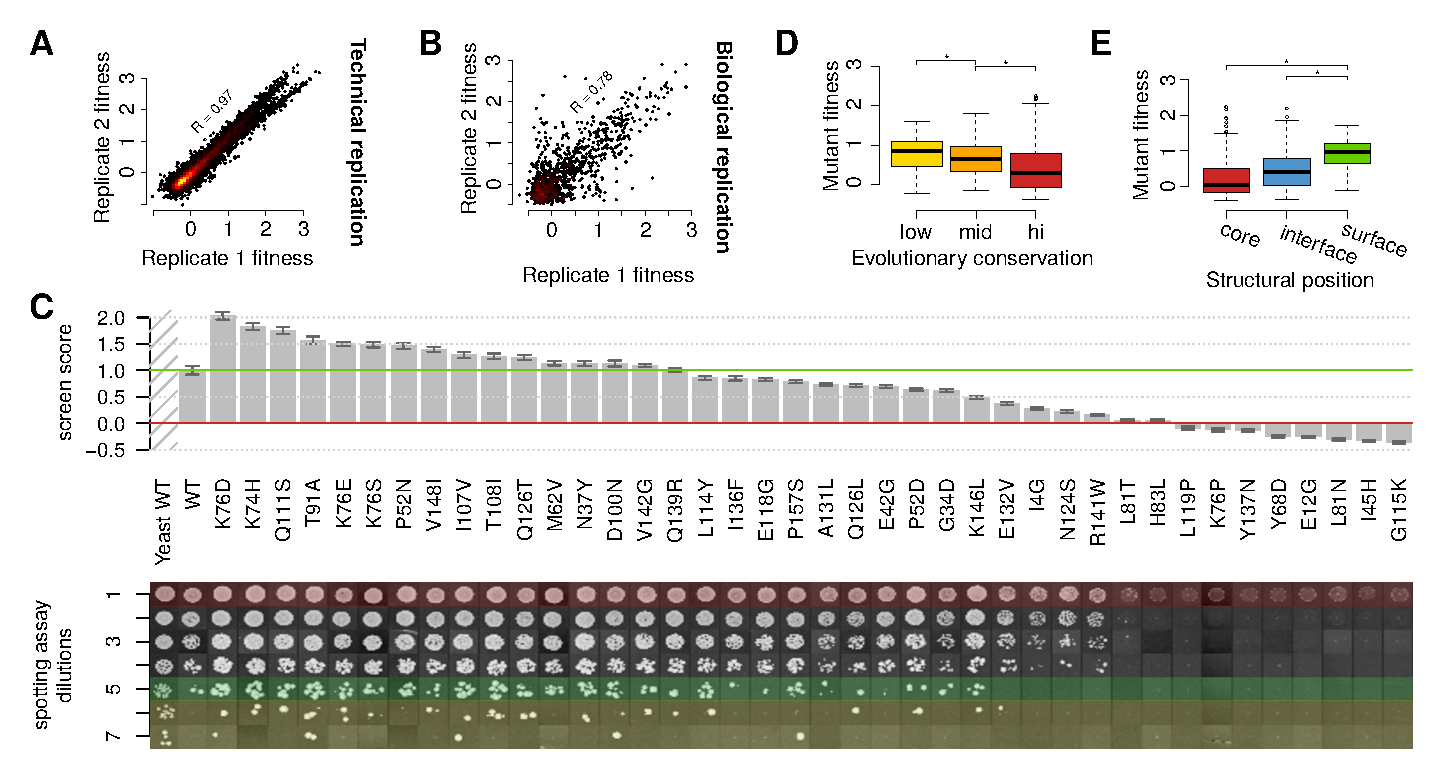
\includegraphics[width=9in]{img/barseq-validation.pdf}
	\caption{Validation of DMS-BarSeq of UBE2I. A: Correlation between technical replicates B: Correlation between biological replicates. C: Manual complementation spotting assay compared to DMS fitness measurements. D: Comparison of fitness levels for mutations at positions with low, medium and high evolutionary conservation. E:Comparison of fitness levels for mutations at positions within the hydrophobic core, at interaction interfaces, and unused surfaces}
	\label{fig:barseqValidation}
\end{figure}
\end{landscape}


\subsubsection{An alternative strategy for DMS via tiled regional sequencing}

While the DMS-BarSeq approach has many advantages (see Discussion), its performance comes at the cost of producing and maintaining an arrayed clone library, and of determining the full-length sequence of each coding region and barcode for each clone. We therefore investigated an alternative approach called DMS-TileSeq: Instead of tracking the fitness of each individual clone, we carried out en masse measurements of the frequency of each variant in the pool before and after selection, by deep sequencing.  Sequencing was carried out for a set of short amplicon tiles that collectively encompass the complete coding region.  In this way, we can discern the impact of each mutation by observing the impact of selection on the abundance of clones carrying this mutation.

In terms of mutagenesis (Stage 1), DMS-TileSeq is identical to DMS-BarSeq.  Given the mutagenized amplicon library, the cloning step (Stage 2) was carried out by \textit{en~masse} recombinational subcloning into complementation vectors (thus skipping the step of arraying and sequencing individual clones).  This plasmid pool was next transformed en masse into the \textit{ubc9-ts} strain appropriate for assessing the complementation ability of UBE2I variants. As with DMS-BarSeq, DMS-TileSeq employs pooled strains grown competitively (Stage 3) at the permissive and selective temperatures. However, instead of using barcode sequencing to determine the fitness associated with individual stains, we directly sequence the coding region from the clone population to determine the frequency of each variant in each pool (before and after selection). To overcome the problem of distinguishing mutations from sequencing errors, we divide the coding region into tiles such that each individual template molecule can be completely sequenced on both strands.  By requiring that each variant be seen on both strands, the incidence of base-calling errors can be substantially reduced6.  DMS-TileSeq requires that the library be sufficiently complex to ensure that the effect of a mutation is determined from enough clones and over enough genetic backgrounds (where there are multiple variants per clone) to be reproducible (see Online Methods).

To validate the reliability of DMS-TileSeq, we first applied it to UBE2I and compared the results with those obtained using DMS-BarSeq. Correlation between DMS-TileSeq and DMS-BarSeq was comparable to the correlation observed between biological replicates of DMS-BarSeq (Supplementary Figure 2), suggesting that reproducibility of DMS-TileSeq is at least comparable to that of DMS-BarSeq. DMS-TileSeq and DMS-BarSeq showed comparable agreement with complementation scores from manual assays (Supplementary Figure 3).  Thus, DMS-TileSeq avoids the substantial cost of arraying and sequencing thousands of individual clones, while performing on par with DMS-BarSeq in terms of reliability of the functional complementation scores it produces.

\begin{figure}[h!]
	\centering
	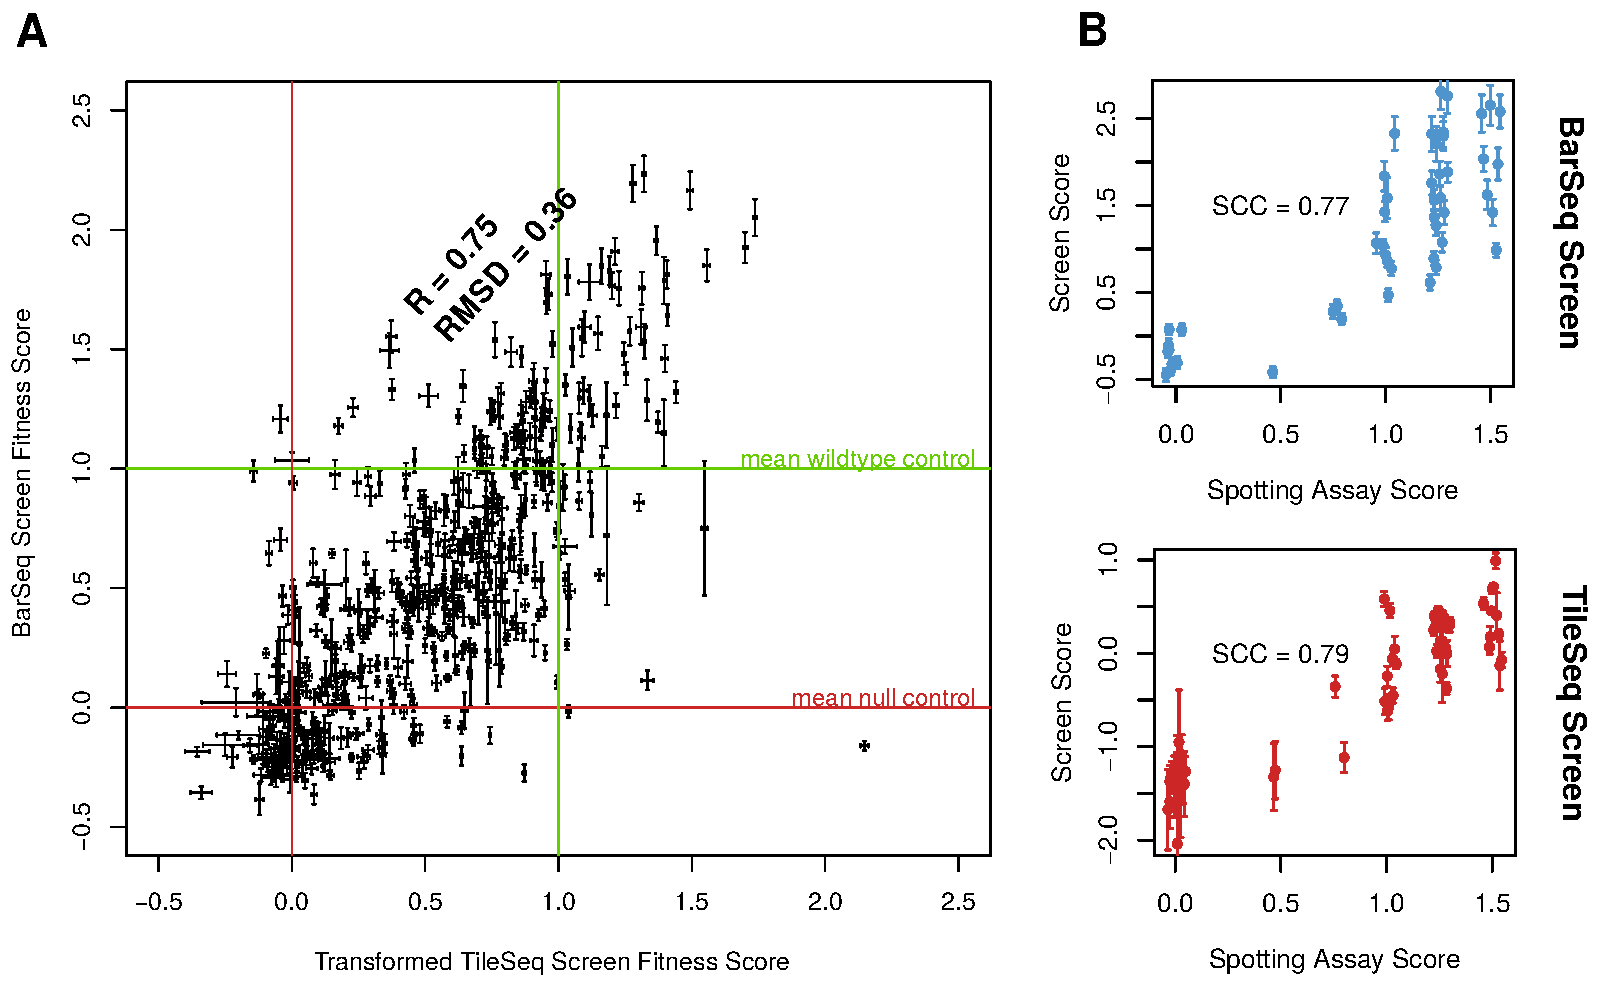
\includegraphics[width=.7\textwidth]{img/barVtile.pdf}
	\caption{Comparison of BarSeq to TileSeq scores. }
	\label{fig:barVtile}
\end{figure}

\subsection{A complete functional map of UBE2I}

Having performed two independent deep mutational scans of UBE2I using functional complementation assays, we wished to integrate both results into a single comprehensive high-quality map. To accomplish this, we first combined the results of each screening approach into a joint map.  This required bringing the maps onto the same scale. Using a regression-based transformation function, we transformed the DMS-TileSeq scores to the more intuitive scale of DMS-BarSeq (where 0 corresponds to the typical score of a null mutant and 1 corresponds to the typical score of a wildtype control). We then combined scores from the two methods, giving greater weight to more confident measurements (see Online Methods).

\subsubsection{Imputation and regularization of missing or less accurate data}

As is the case for all previously published DMS maps, our combined map contained some entries that were poorly measured or missing (e.g., because these substitutions were underrepresented in the input clone library). To fill the gaps in the map (Stage 5 in the framework), we trained a random forest~\cite{17} regression model using the existing measurements in the map. The features used for the model fall into four categories: intrinsic information; conservation information; chemicophysical properties; and structural properties. The most important intrinsic feature consists of weighted positional averages in the map. That is, for any given amino acid change, we weight all other observed effects of variants at the same amino acid position by their measurement confidence and form the average. A second intrinsic feature consists of the confidence-weighted average effect of all variants containing the amino acid change in question. Finally, as a third intrinsic feature we calculate the expected variant fitness predicted by a multiplicative model often applied to detect genetic interactions~\cite{18}. The model is applied to all available double mutants fitness values carrying the mutation in question in combination with available complementary single mutant fitness values. As the latter two features rely on multi-mutant fitness measurements, they can only be applied where DMS-BarSEQ data is available. The second category of features describes evolutionary conservation. For each amino acid change in question this encompasses the corresponding BLOSUM62~\cite{19}, SIFT~\cite{20} and PROVEAN~\cite{15} scores, and the AMAS~\cite{21} conservation at the given position. The third set of features comprises chemicophysical properties such as mass and hydrophobicity of  the original and wildtype amino acids and the difference between the two. The fourth and final set of features consisted of structural properties of the affected amino acid residues, such as solvent accessibility and burial in interaction interfaces.

We assessed the performance of the imputation model using cross-validation. Surprisingly, we found the root-mean-squared deviation (RMSD) of imputed values to be on par with measurement error in experimentally measured data (Supplementary Figure S3A). An examination of the prediction performance by location showed increased error in positions with lower mutation density and for variants with in above-WT fitness levels (Supplementary Figure S3B). As an additional validation step, we performed manual complementation assays for a set of UBE2I variants that were not present in the machine learning training data set and compared the results against the predictions (Supplementary Figure S3C), again finding a surprisingly strong agreement. Notably however, variants showing above wild-type level growth in the manual assay

\begin{landscape}
\begin{figure}[h]
	\centering
	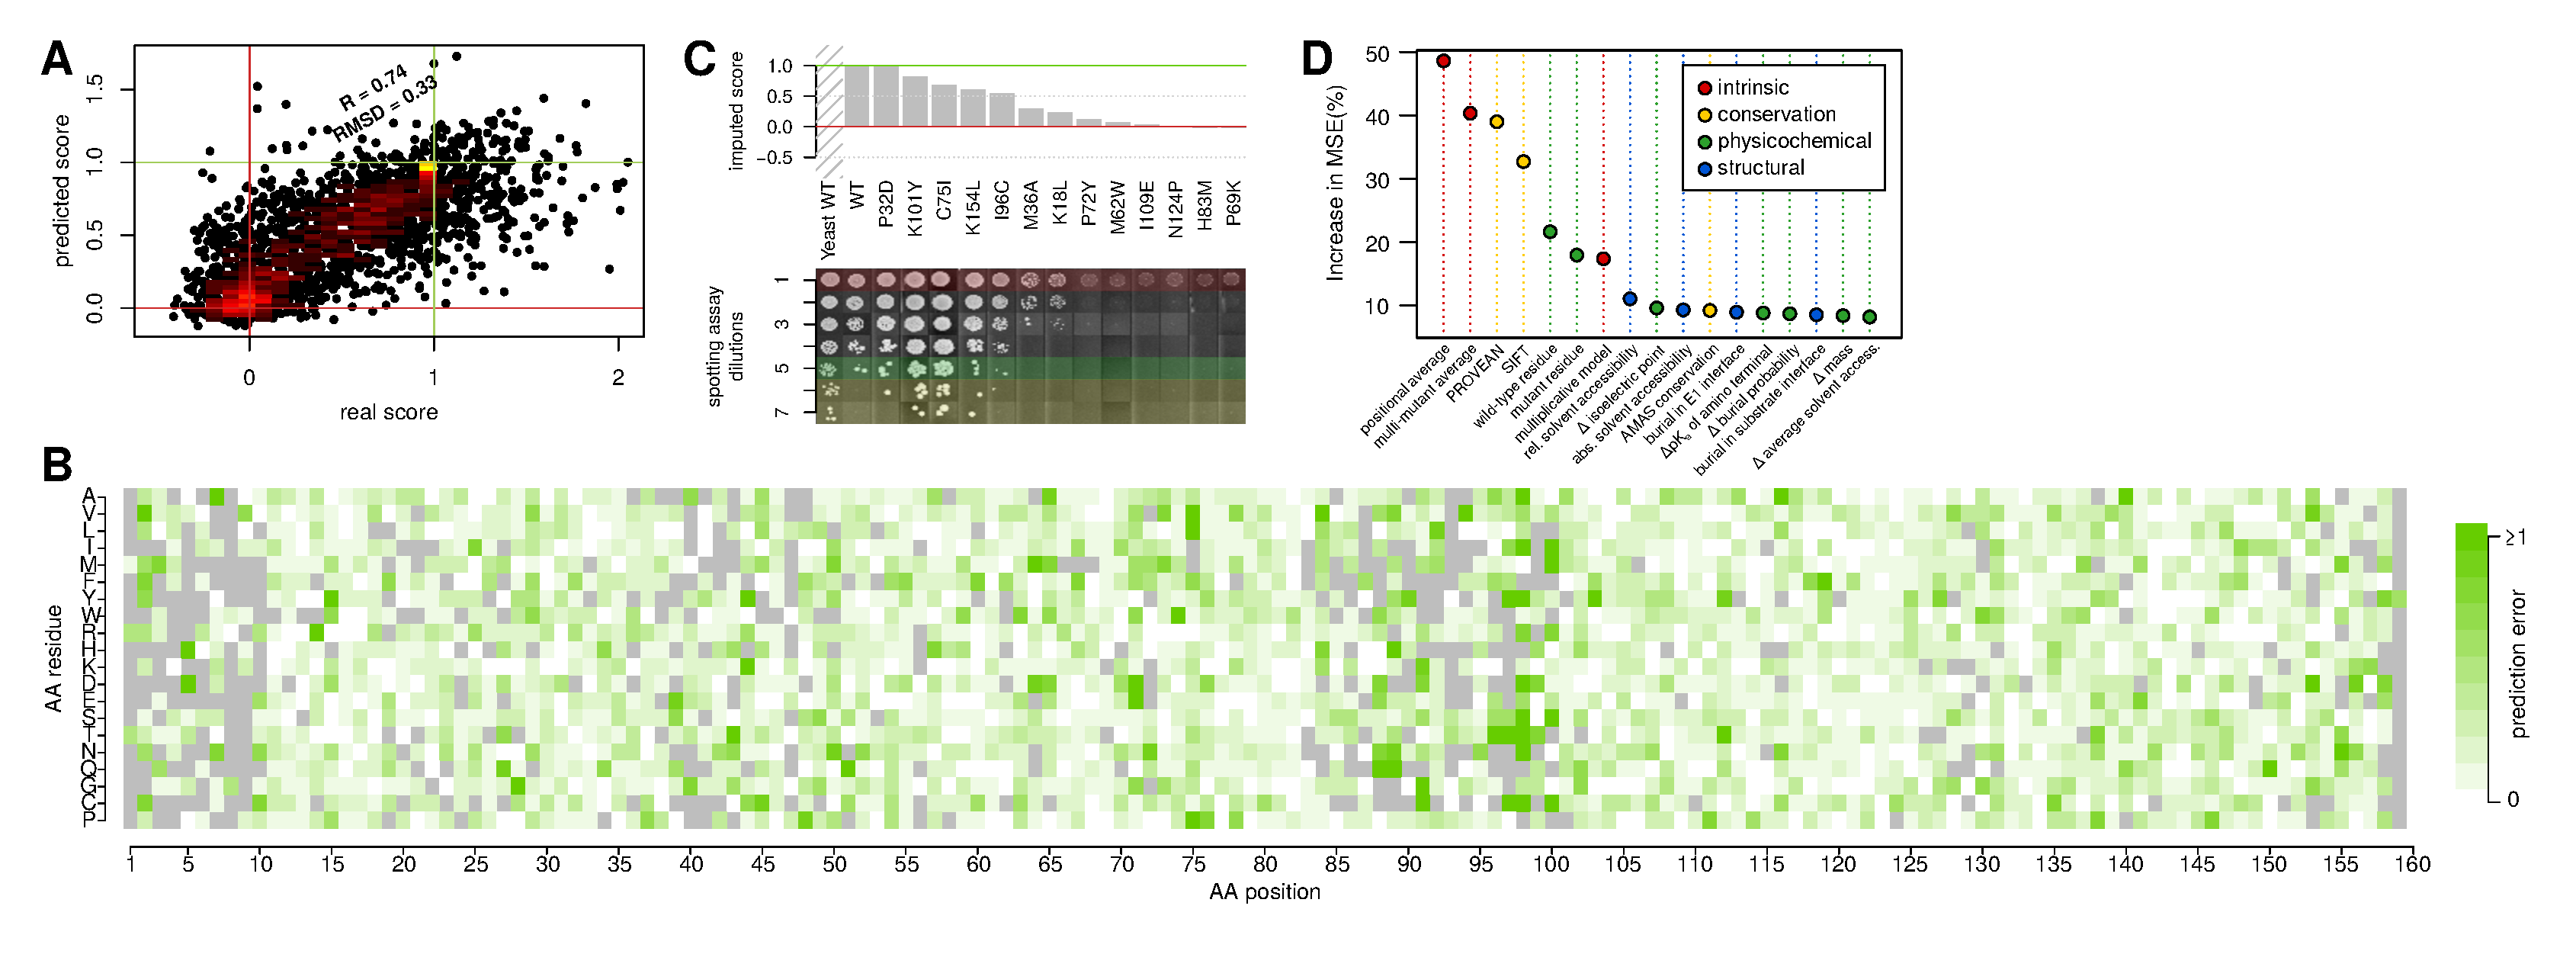
\includegraphics[width=9in]{img/imputation.pdf}
	\caption{Evaluation of Machine learning imputation. A) Cross-validation correlation between measured values and machine learning predictions. B) Cross validation prediction error landscape. C) Manual complementation spotting assay compared to machine learning predictions for an independent test set of variants not present in the training data. D) Feature importance as measured by average increase in mean squared error.}
	\label{fig:imputation}
\end{figure}
\end{landscape}

Finally, towards stage 6 of the framework, we wished to address cases in which experimental measurements were available but less confident. We employed a regularization method, combining experimental measurements with machine-learning predicted values after dynamically weighting them according to their respective confidence levels. That means: the less confident a measurement, the stronger the regularization. 

\todo{At this point it would be nice to show off the value of the regularization, but for the unflipped UBE2I map it doesn’t improve anything. The flipped maps, especially for TPK1 and CALM1 benefit much more from regularization. It would also be great if we could point to the spotting assay, but we didn’t test any poorly measured clones, so we don’t have any interesting data there.}

The complete, refined functional map of UBE2I after imputation and regularization can be seen in Figure 2A. To evaluate the complete map, we once more applied manual complementation assays to a set of variants that represented the full range of fitness scores.  DMS fitness scores corresponded closely with manual assays (Supplementary Figure S4A), thus validating our framework.  To more specifically evaluate the imputation process, we selected a smaller test set of variants (again spanning the range of scores), and recalculated imputation scores using a training set that excluded variants in this test set.  Collectively, our framework yielded a comprehensive map covering all possible missense variants, with overall quality that was on par with the highest-quality measurements from either screen alone.

\subsection{Evaluation and validation of the UBE2I map}

\section{Methods}

\section{Discussion}

